\section{System Overview}
The system comprises an input hopper, feed guides, an indexing mechanism (cam or Geneva), a counting gate, a binding station, and an output collection tray. Drive power is provided by a hand crank or small motor coupled through gears to achieve the required torque and speed.
\section{Sequence of Operations}
A block diagram represents the functional flow (Fig. \ref{fig:functional-flow}). Each block is coordinated by the indexing cycle to ensure one-to-one correspondence between counts and bindings.
\vspace{1ex}

Iterative adjustments will be made based on test results to optimize performance and reliability. Flow charts (Fig. \ref{fig:design-analysis}) will be used to validate the sequence of operations and identify potential failure points for mitigation.
% \begin{figure}[!htbp]
% \centering
% 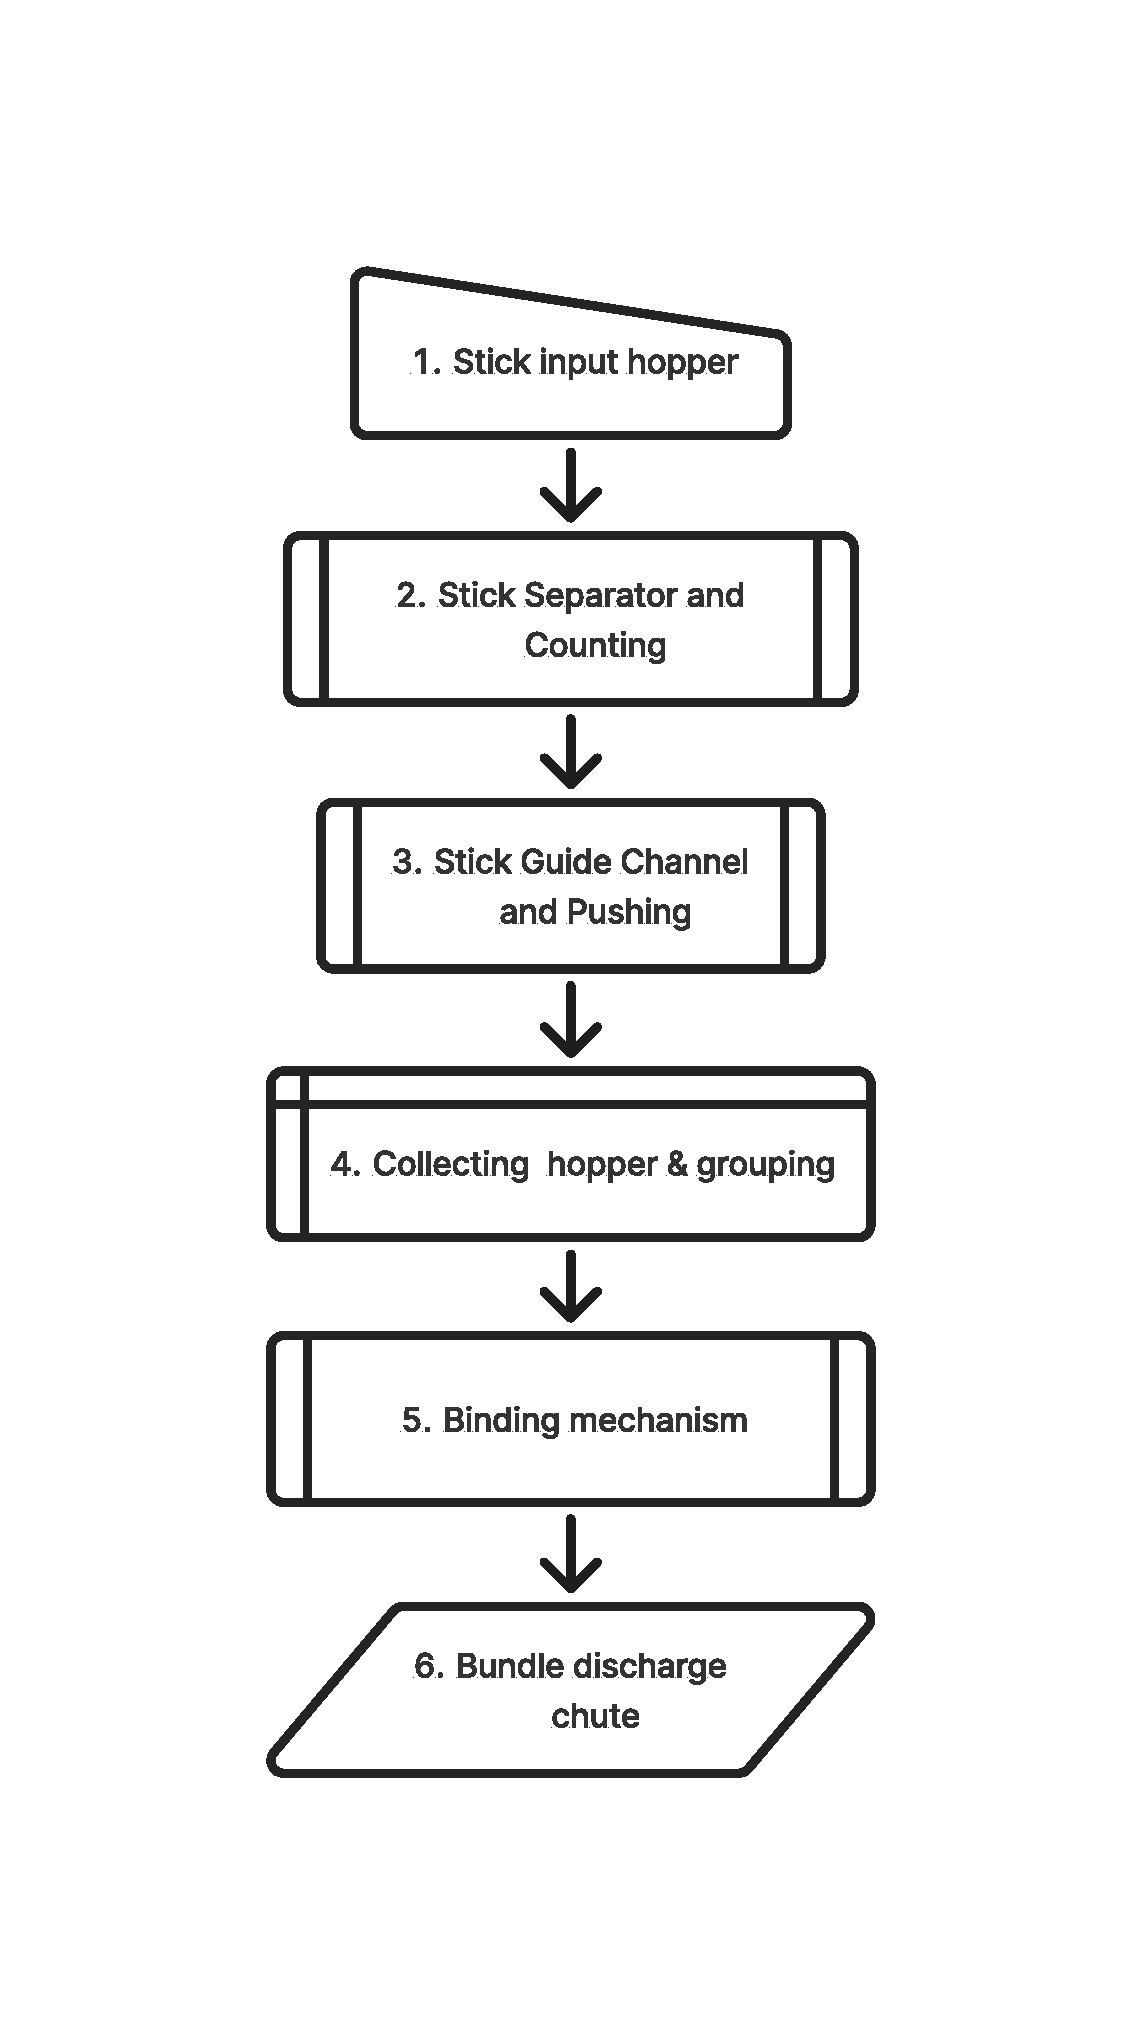
\includegraphics[
%   width=\textwidth,
%   height=0.5\textheight,
%   keepaspectratio
% ]{images/functional-flow.pdf}
% \caption{Functional block diagram of the mechanical counting and bundling machine.}
% \label{fig:functional-flow}
% \end{figure}

\section{Overall Design and Analysis Workflow}

Design and analysis will begin with concept generation and selection, followed by detailed kinematic design of the indexing mechanism. CAD modeling will be used to refine the design, followed by kinematic and dynamic analysis and finally testing and documentation. 

Iterative adjustments will be made based on test results to optimize performance and reliability. Flow charts (Fig. \ref{fig:design-analysis}) will be used to validate the sequence of operations and identify potential failure points for mitigation.

\begin{figure}[!htbp]
    \centering
    % Left Figure
    \begin{subfigure}[b]{0.46\textwidth}
        \centering
        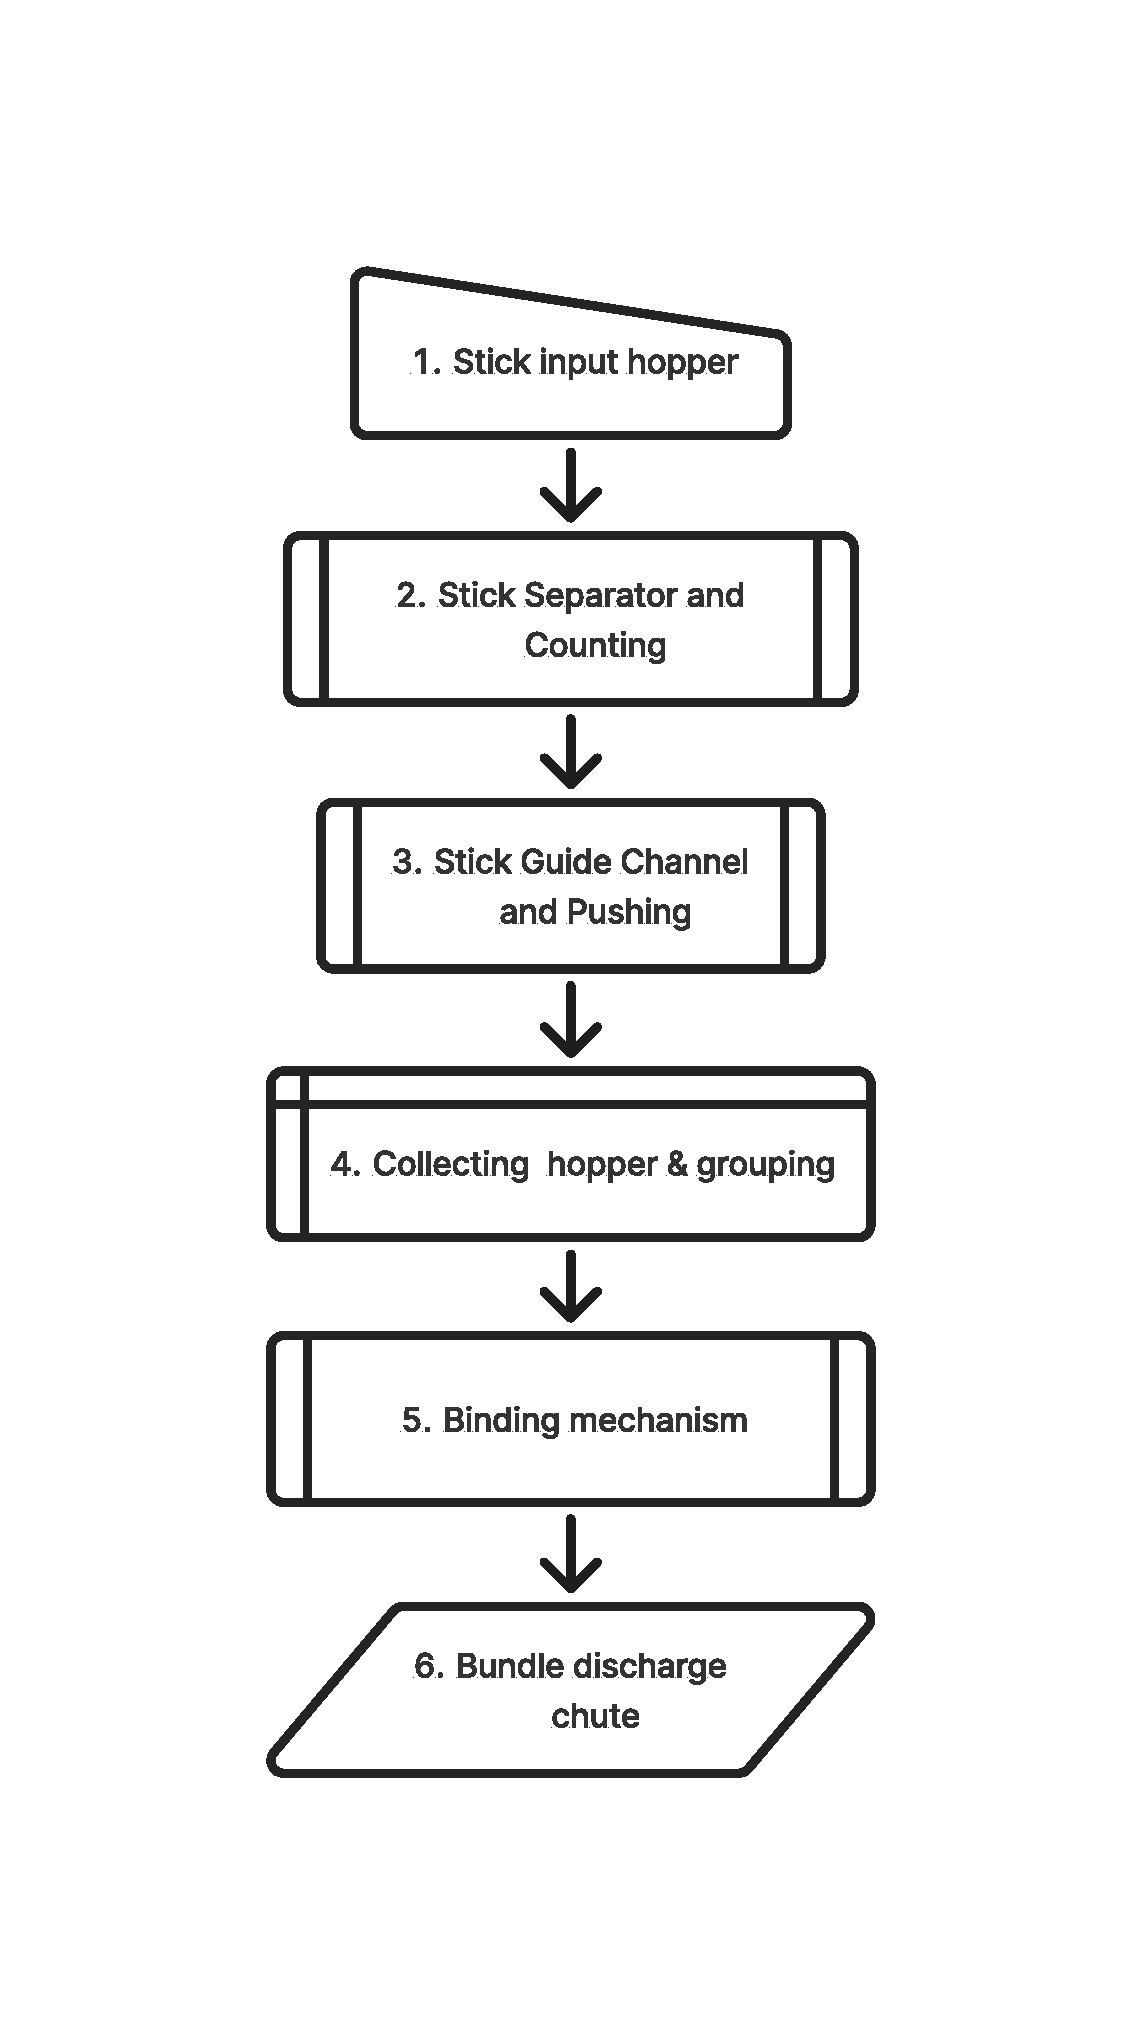
\includegraphics[width=\textwidth, height=0.8\textheight, keepaspectratio]{images/functional-flow.pdf}
        \caption{Functional block diagram of the mechanical counting and bundling machine.}
        \label{fig:functional-flow}
    \end{subfigure}
    \hfill % Adds horizontal space between the two figures
    % Right Figure
    \begin{subfigure}[b]{0.46\textwidth}
        \centering
        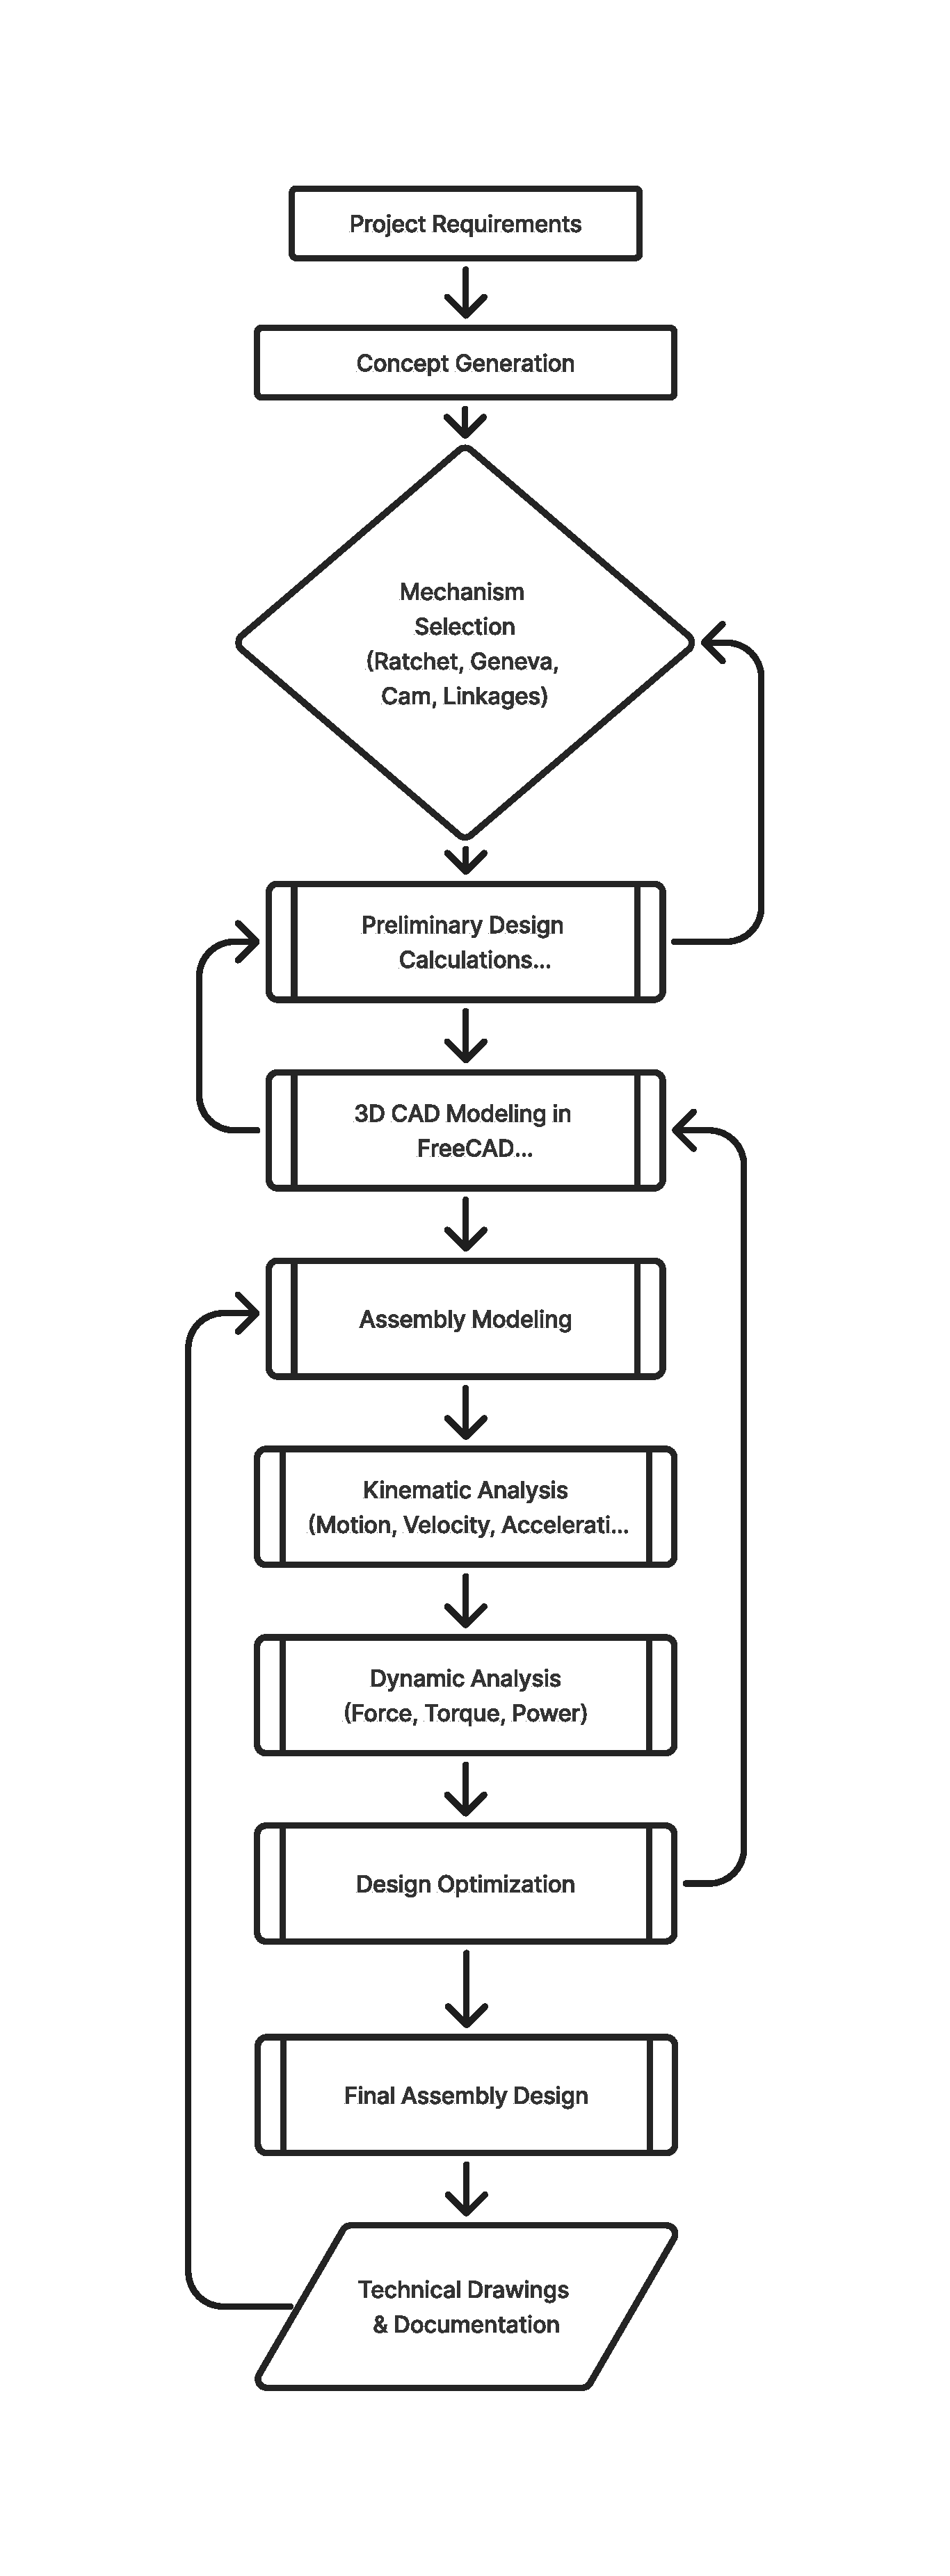
\includegraphics[width=\textwidth, height=0.8\textheight, keepaspectratio]{images/design-analysis.pdf}
        \caption{Flow chart depicting the sequence of operations and decision points for the mechanical counting and bundling machine.}
        \label{fig:design-analysis}
    \end{subfigure}
    
    % Optional: Overall main caption for both figures combined
    \caption{System block diagram and process flowchart.}
\end{figure}


\section{CAD Modeling and Simulation}
CAD software (SolidWorks) will be used for 3D modeling of the mechanism, allowing for detailed design and interference checks. Kinematic analysis will be performed to ensure the desired motion profiles are achieved, while dynamic analysis will evaluate forces and stresses to inform material selection and structural design. Simulation results will be validated against theoretical calculations to ensure accuracy and reliability of the design before prototyping. Flow chart \ref{fig:cad-wrokflow} shows a typcial .

\begin{figure}[!htbp]
	\centering
	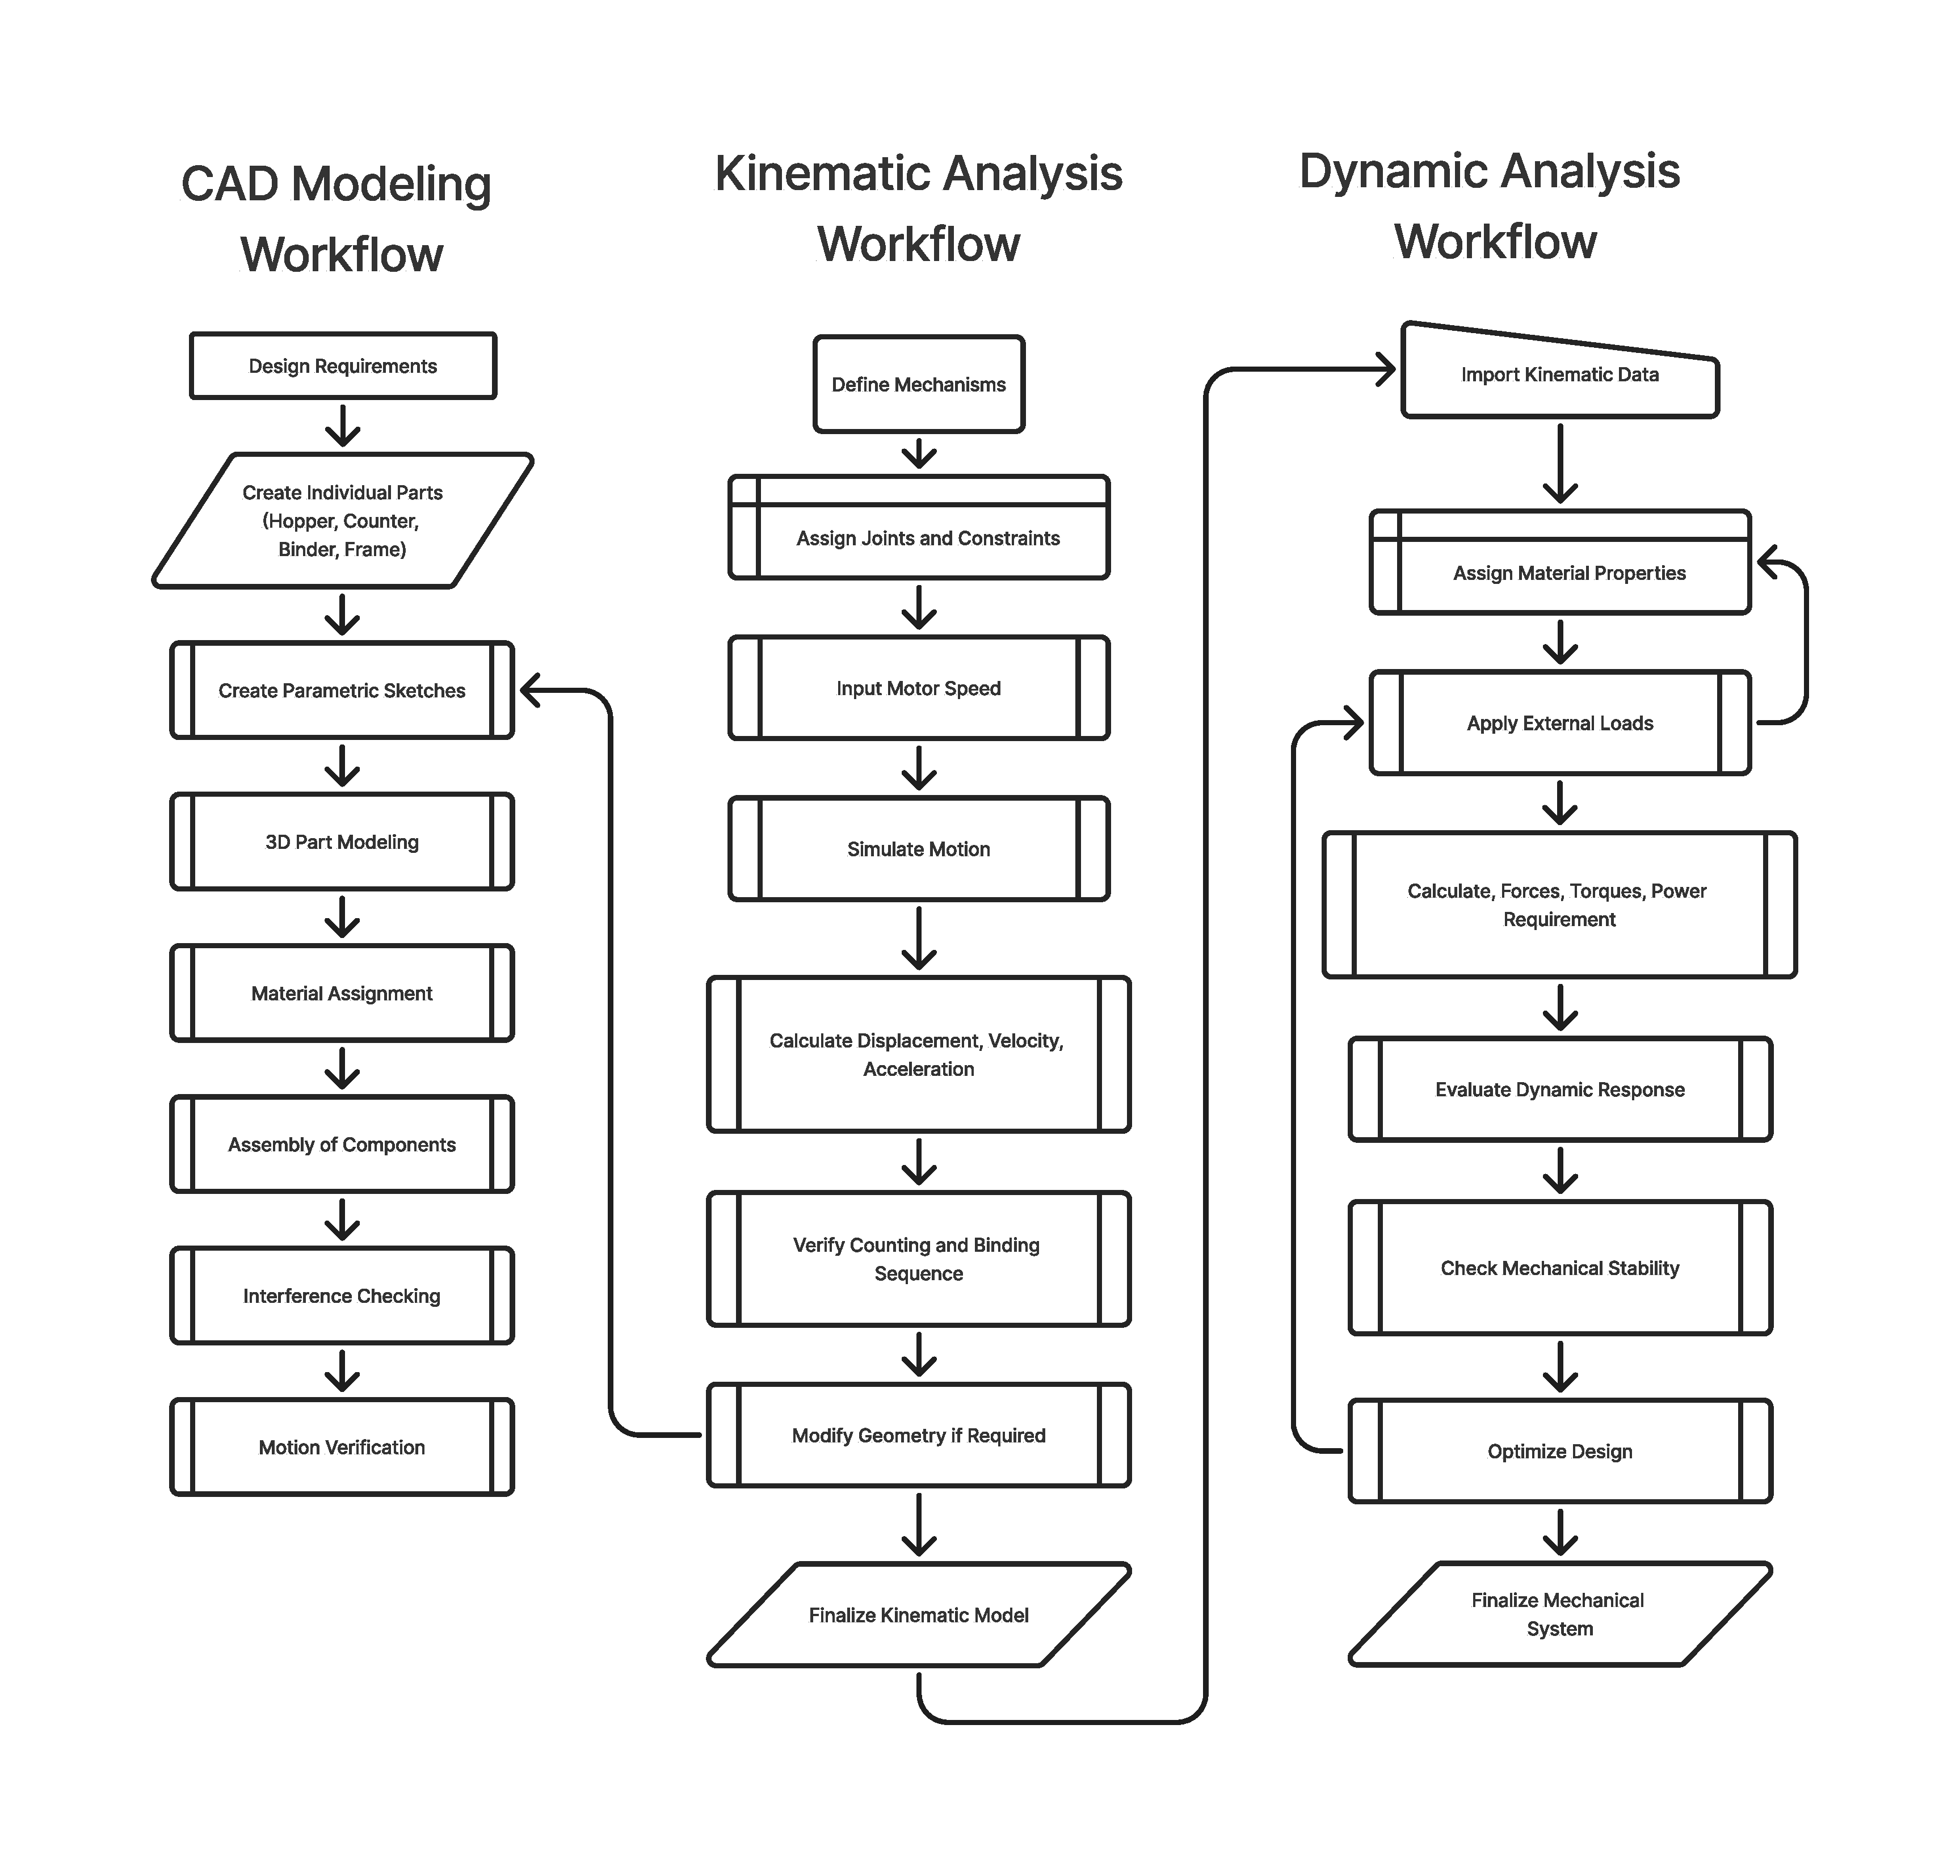
\includegraphics[width=\textwidth, height=0.8\textheight, keepaspectratio]{images/cad-workflow.pdf}
	\caption{Flow chart illustrating the CAD modeling and simulation workflow for the mechanical counting and bundling machine.}
	\label{fig:cad-wrokflow}
\end{figure}
